% IEEE Paper Template for US-LETTER Page Size (V1)
% Sample Conference Paper using IEEE LaTeX style file for US-LETTER pagesize.
% Copyright (C) 2006 Causal Productions Pty Ltd.
% Permission is granted to distribute and revise this file provided that
% this header remains intact.
%
\documentclass[10pt,conference,letterpaper]{IEEEtran}
\usepackage{times,amsmath,epsfig}

%
\usepackage{makeidx}  % allows for indexgeneration
%
\usepackage{graphicx}
\usepackage{stfloats}
\usepackage{amsmath}
\usepackage{bbm}
\usepackage{amssymb}
\usepackage{multirow}
\usepackage{mathrsfs}
\usepackage{url}
\usepackage{listings}
\usepackage{color}
\usepackage{wrapfig}
\usepackage{mathtools}
 
\usepackage{algorithm}
\usepackage{algorithmic} 

\lstloadlanguages{XML}

\newcommand{\beq}{\begin{equation}}
\newcommand{\enq}{\end{equation}}
\newcounter{mytempeqncnt}
\newcommand{\bquote}{\begin{quote}}
\newcommand{\equote}{\end{quote}}

\newcommand{\todo}[1]{\textcolor{red}{@TODO: #1}}
\newcommand{\dtr}[1]{\textbf{\textit{#1}$^\textbf{[dtr]}$}}
\algsetup{linenosize=\small}
\newtheorem{definition}{Definition}
 
\title{Efficient and Effective On-line Learning-Based Instance Matching over Heterogeneous Data}
%
\author{%
% author names are typeset in 11pt, which is the default size in the author block
{Samur Araujo{\small $~^{\#1}$}, Duc Thanh Tran {\small $~^{*2}$}, Arjen de Vries{\small $~^{\#3}$} }%
% add some space between author names and affils
\vspace{1.6mm}\\
\fontsize{10}{10}\selectfont\itshape
$~^{\#}$Delft University of Technology, PO Box 5031, 2600 GA Delft, the Netherlands\\
\fontsize{9}{9}\selectfont\ttfamily\upshape
$~^{1}$s.f.cardosodearaujo@tudelft.nl\\
$~^{3}$a.p.devries@tudelft.nl%
% add some space between email and affil
\vspace{1.2mm}\\
\fontsize{10}{10}\selectfont\rmfamily\itshape
$~^{*}$Karlsruher Institute of Technology, Germany\\
\fontsize{9}{9}\selectfont\ttfamily\upshape
$~^{2}$ducthanh.tran@kit.edu
}
%
\begin{document}
\maketitle
%
\begin{abstract} 
This document gives formatting instructions for authors preparing
papers for publication in the Proceedings of an IEEE conference.  The
authors must follow the instructions given in the document for the
papers to be published.  You can use this document as both an
instruction set and as a template into which you can type your own
text.
\end{abstract}

% NOTE keywords are not used for conference papers so do not populate them
\begin{keywords}
ignore
\end{keywords}
   
%\section{Introduction}
\emph{Instance matching} \cite{DBLP:journals/ijswis/FerraraNS11} refers to the problem of determining whether two descriptions are about the same real-world entity. Traditionally, research in this context was focused on the single-domain setting, where data come from the \emph{same or similar datasets}. Basically, given the descriptions of entities available as records in databases, RDF descriptions on the Web, etc., the instance matching task breaks down to the core problems of (1) finding a suitable \emph{instance representation} (i.e., selecting attributes and their values), (2) using this for evaluating different \emph{similarity measures}, and (3) finally selecting the most similar ones according to a \emph{threshold}. 
%To sum up, the instance matching problem lays on efficiently finding candidate matches and effectively assigning the correct matches. 

For large datasets, the instance matching problem is typically solved in two steps, namely to find candidate matches first using a relatively simple but quick matching technique, and then to refine them using a more advanced but also more expensive technique. For the latter more sophisticated and \emph{effective matching}, there are different techniques for learning the right combination of attributes, similarity measures and threshold to be used for computing and selecting the resulting matches~\cite{DBLP:conf/cikm/SongH10,MaurouxHJAM09,nikolov08}. Typically, the former, \emph{candidate selection} resembles what is called  \emph{blocking}~\cite{hernandez_merge/purge_1995,MichelsonK06,elmagarmid_duplicate_2007} in the single dataset settings (e.g. deduplication), which is described as the process of finding non-overlapping blocks of instances that share a similar key (a compact description of an instance), such that they can be compared between each other. For this type of key matching, indexes can be built to accelerate the process. In particular, fast \emph{index lookups} can be performed to directly retrieve candidates from the index that share/overlap with the key of a given source instance. 

%For instance, given an instance and the value tokens \verb+Anemia+ appearing in its \verb+name+ attribute as key, candidates for this instance can be obtained via an index lookup, which simply returns all instances with \verb+Anemia+ as name. 
%Given two datasets with $n$ and $m$ elements respectively, candidate selection requires only $n$ lookup queries over the index built for the $m$ elements (for retrieving candidate blocks for $n$ elements), while $n\times m$ similarity computation steps are needed for the effective matching of instances between these datasets. 

In this work, we focus on the problem of candidate selection in the Web environment with \emph{multiple heterogeneous datasets}, such as Linked Data. Here, heterogeneity particularly means that the datasets' schemas might vary. Existing techniques~\cite{MichelsonK06} assume instances are from the same or similar datasets such that the keys chose for one dataset can also be used to find candidates in the other datasets. This is however problematic in this setting because for a key such as one based on the values of the \verb+name+ attribute in the one dataset, there might not exist the \verb+name+ attribute, in the other datasets. Aiming to address this problem of heterogeneity, schema-agnostic candidate selection has been proposed recently~\cite{papadakis_efficient_2011}. It does not exploit attributes for building keys, but instead, simply treat instances as unstructured bags of tokens that can be extracted from the attribute values. That is, the key is simply composed of set of tokens that do not come with any attribute information. Instances are considered similar and form blocks when their keys overlap, i.e. they have some tokens in common. The drawback of the schema-agnostic approach is that it may build very ambiguous candidate sets, because a token may not be discriminative enough. For instance, the token "Paris", occurs in 7446 distinct instances at DBPedia\footnote{http://dbpedia.org/} dataset. 
%We illustrate the heterogeneity problem and the drawbacks of the schema-agnostic approach to that using the following example: 

%\begin{example}
%There are two descriptions of the \verb+anemia+ disease that were extracted from two different datasets. The first one is the Diseasome dataset, which specifically represents data from the Life Science domain. The second one is DBpedia, a cross-domain encyclopedic type of dataset.  
%While the description from Diseasome describes genetic aspects (Fig. 1, line 1), the one from DBpedia captures general aspects (Fig. 1, line 7) of \verb+anemia+. The only token they have in common is ``Anemia'', while their schemas do not overlap at all. Applying blocking techniques that use attributes to form keys~\cite{DBLP:conf/semweb/SongH11} is not directly possible because there are no common attributes shared by these datasets. Using schema-agnostic blocking that compares instances simply by value tokens, these instances can be identified to be candidate matches. However, this token match is not enough to guarantee these instances refer to the same disease, because this blocking may yield other candidates, such as \verb+anemia+ as a plant, as shown in Fig. 1, line 12. 
%\end{example}

%\begin{figure} 
 
%\centering
%\includegraphics[width=0.8\textwidth]{fig1.png}
%\caption{Examples for ``Anemia'' in N3 notation (prefixes are used for brevity).} 
%\vspace{-10pt}
%\end{figure} 

We note that there exist only a few works~\cite{DBLP:conf/semweb/SongH11,papadakis_efficient_2011} that specifically address the problem of candidate selection over multiple heterogeneous datasets. To this end, this work provides the following contributions: 

\textbf{Effective Candidate Selection}. Schema-agnostic candidate selection looses valuable attribute information and thus may yield too many candidates. On the other hand, using attributes to form keys requires schema matching\cite{DBLP:conf/ic3k/ScharffeE11} to find attributes in one dataset that correspond to (key) attributes in the other dataset~\cite{DBLP:conf/semweb/SongH11}. 
%As illustrated by the example, attribute matches between datasets may not exist. 
In this work, we exploit attribute information for more effective candidate selection. However, we do not require attributes to complete match (e.g. "surname" and "family name") but employ a more relaxed notion of \emph{comparability} (e.g. we may map "drugname" and "synomym"). In particular, even when they represent completely different attributes, some pairs of attributes among them might be more comparable than some other pairs. The comparability between attributes is then used to construct lookup queries on the target dataset. In order to obtain a high recall (i.e. retain correct candidates, true positives), which is the topmost goal in candidate selection, all comparable attributes have to be considered for constructing the queries. Among them, there exists a group that return the best set of candidates. We propose a \emph{branch-and-bound based optimization framework} that iteratively search for this optimal query. 

\textbf{Efficient Candidate Selection}. 
%We also show that schema-agnostic candidate selection is not efficient as queries built from values without attribute information. They match a large number of instances, resulting in a large amount of data that has to be loaded from disk. 
Using attribute-value pairs in the keys increases the selectivity of the resulting queries. However, since all comparable attributes are considered for achieving high recall, we obtain a large amount of candidate queries. To also optimize for efficiency, we incorporate the number of queries and query execution times into the branch-and-bound optimization so that it is geared not only towards queries that produce high quality results but also, towards executing a minimal number of time-efficient queries. 

In the experiments, we show that compared to the schema-agnostic~\cite{papadakis_efficient_2011} and the schema-based~\cite{DBLP:conf/semweb/SongH11} approaches, our approach yields superior results both in terms of efficiency and effectiveness in 96\% of the cases. We compare our approaches on the context of instance matching itself, showing that it produces competitive results to other systems that approach the problem on off-line fashion.

\textbf{Outline.} 
This paper is organized as follows. After this introduction, we present the problem of candidate selection over multiple heterogeneous datasets, in the Section 2. In Section 3, we elaborate on our algorithm for building candidate selection queries. In Section 4, we present the algorithm to find candidate sets itself.  Section 5 presents the experimental results, along with a comparative study against two known state-of-the-art approaches for candidate selection. Section 6 introduces the related work. Finally, Section 7 concludes this paper.

 

\section{Overview}
In this section, we introduce the data model, discuss the problem, and finally, present a brief overview of existing solutions as well as our approach.

\subsection{Data} We focus on heterogeneous Web data including relational data, XML, RDF and other types of data that can be modeled as graphs. Closely resembling the RDF data model, we employ a graph-structured data model where every dataset is conceived as a graph $G \in\mathbb{G}$ comprising a set of triples: 

\begin{definition}[Data Model] A dataset set is a graph $G$ formed by a set of triples of the form $(s, p, o)$ where $s \in U$ (called subject), $p \in U$ (predicate) and $o \in U \cup L$ (object). Here, $U$ denotes the set of Uniform Resource Identifiers (URIs) and $L$ the set of literals. Every literal $l \in L$ is a bag of tokens, $l = \{t_1,\ldots,t_i,\ldots,t_n\}$, drawn from the vocabulary $V$, i.e. $t_i \in V$.  
\end{definition} 

With respect to this model, \emph{instances} are resources that appear at the subject position of triples. An instance representation can be obtained from the data graph as follows:

\begin{definition}[Instance Representation] The instance representation $IR: U \times \mathbb{G} \rightarrow \mathbb{G}$ is a function, which given an instance $s \in U$ and a graph $G \in \mathbb{G}$, maps $s$ to a set of triples in which $s$ appears as the subject, i.e. $IR(s) = \{ (s, p, o) | (s, p, o) \in G, o \in L \}$. 
\end{definition} 

Thus, an instance is basically represented through a set of \emph{predicate-value} pairs, where values are bags of tokens. \todo{add a graph to provide example, also, provide one example for instance representation} 
We will use the terms instance and instance representation interchangeably from now on. Note that for the sake of presentation, only the outgoing edges $(s, p, o)$ of an instance $s$ are considered while incoming edges (triples where $s$ appears as the object) can also be added to the representation of $s$. 

\subsection{Problem - Find Instance Matches and Match Candidates} \emph{Instance matching} is about finding instances that refer to the same real-world object based on their representations extracted from the data. In this paper, we tackle the problem of \emph{instance matching across multiple datasets}: given instances of a \emph{source dataset} $G_s$, the problem is to find instances in others datasets, collectively referred to as the \emph{target dataset} $G_t$, which represents the same real world object. 

\textbf{Challenges.} Compared to the single dataset setting, this problem entails additional challenges especially when the data is heterogeneous not only at the data but also schema level. In this regard, \emph{data-level heterogeneity} means that for the same property, instances referring to the same object may have different values, or different syntactical representations of the same value. \todo{For instance, the values "Michael Jackson" or "Jackson, Michael" can be both used as the value of the property name of an instance representing  Michael Jackson.} (1) \emph{Schema-level heterogeneity} arises when there is only little or no schema overlaps between the datasets. That is, instances referring to the same object may be represented by different predicates, or different representations of the same predicates. Finding different representations of the same predicate is part of a problem also known as schema matching. Another challenge in this multiple dataset setting is (2) \emph{efficiency}: for instance matching, a scheme is needed to determine how to compare two given instances; we will show that especially with schema heterogeneity, finding the best scheme for matching across heterogeneous datasets involves a greater search space and more feedback information (training data). Searching through all possible solutions and obtaining feedback information to evaluate them is expensive especially when we consider the online learning of instance matching schemes that requires access to data from remote endpoints. \todo{discuss in intro that we need schemes for individual instances, and motivates and explain the concept of online learning of instance schemes: involves live access to remote endpoints that host fresh version of the datasets.}

\textbf{Computing Instance Matches.} More precisely, an \emph{instance matching scheme} is a (weighted) combination of similarity function predicates, $\sum_i{w_i \sim(p_i)} > \alpha$.  Every $\sim(p_i)$ is a function, which given two instances $s_i$ and $s_j$, returns the similarity between these instances based on their similarity on the values of the predicate $p_i$. The scheme computes the overall similarity between $s_i$ and $s_j$ by combining the similarities obtain for individual predicates and determines them as a \emph{match} when its exceeds the threshold $\alpha$. Clearly, such a scheme focus on data-level heterogeneity. Given $s_i$ and $s_j$ are in the source and target datasets, respectively, and these datasets vary in schema, an extended scheme of the form $\sum_i{w_i \sim(\langle p^s_m,p^t_n \rangle_i )} > \alpha$ is needed to capture that the values of the source predicate $p^s_m$ shall be compared with values of the target predicate $p^t_n$. In other words, when the predicates in the source and target are not the same, comparable pairs of predicates have to be found and incorporated into the scheme. 
%The similarity of $s_i$ and $s_j$ is computed by combining the similarity values obtained for all individual pairs of comparable predicates captured by the scheme. They are considered as a \emph{match} when it .
In fact, this problem entails the subproblems of (A) finding the pair of comparable predicates $\langle p^s_m, p^t_n \rangle$ (schema matching) as well as (B) choosing and (C) weighting them, and determining the (D) similarity functions $\sim$ (e.g. Jaccard distance) and (E) thresholds $\alpha$.  

\textbf{Computing Instance Match Candidates.} Instead of solving all these problems, some instance matching solutions focus on the blocking step, which aims to quickly select candidates matches (hence also referred to as the \emph{candidate selection} step). Instead of using a combination of similarity function predicates, candidate selection simply employs a (conjunction of) blocking key(s), i.e. $\bigwedge \sim(\langle p^s_m,p^t_n \rangle_i)$ (called \emph{candidate selection scheme}), where $\sim$ is a binary function that returns whether the two values of $p^s_m$ and $p^t_n$ match or not. Here, the predicates $p^s_m$ and $p^t_n$ constitute the pair of comparable blocking keys while their values are called \emph{blocking key values} (BKV). Usually, the similarity function is based on exact value matching or value overlap. That is, two instances form a \emph{candidate match} if their blocking key values are the same or overlap on some tokens. 
Mostly, $\sim$ is defined manually such that candidate selection amounts to the problem of (A) finding comparable predicate pairs and (B) choosing the most selective ones as blocking key pairs. 
%Fig. 1 depicts the whole instance matching process described here. This paper focus on the candidate selection part of the problem.
Often, candidate selection is performed as a preprocessing step, producing results that are further refined by a more effective instance matcher that also tunes the weights and threshold to obtain better results. 


%\begin{figure} [ht]
% 
%\centering
%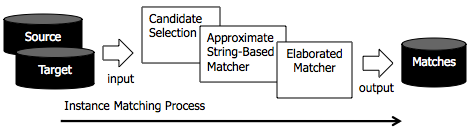
\includegraphics[scale=0.5]{p1.png}
%\caption{Instance matching process overview.} 
%\vspace{-2pt}
%\label{fig:space}
%\end{figure}

 

\subsection{Existing Solutions} 
State-of-the-art matching systems are based on supervised learning, leveraging training data as feedbacks to evaluate candidate schemes~\cite{DBLP:conf/vldb/ChaudhuriCGK07}. Basically, optimal schemes found are those which maximize the coverage of positive examples while avoiding negative examples. They are geared towards homogeneous datasets, focusing on the learning of schemes of the type $\sum_i{w_i \sim(p_i)} > \alpha$ as discussed above. It has been shown that in fact, the underlying learning strategies can also be used to obtain the extended schemes $\sum_i{w_i \sim(\langle p^s_m,p^t_n \rangle_i )} > \alpha$. Instead of all combinations of individual predicates, the search space would have to include all combinations of all possible pairs of predicates. 

Since obtaining representative training data across datasets is difficult, recent approaches that specifically target heterogeneous data derive schemes directly from the data. However, unsupervised approaches of this kind focus on the more simpler problem, namely the learning of the candidate selection schemes $\bigwedge \sim(\langle p^s_m,p^t_n \rangle_i)$. For instance, Song and Heflin~\cite{DBLP:conf/semweb/SongH11} assume precomputed schema mappings such that the comparable predicate pairs are known. They propose to choose them based on their coverage and discriminability; two metrics derived from the data basically reflecting the number of instances a given predicate can be applied to and how well it distinguishes them. Based on manually defined coverage and discriminability threshold, the best pairs of comparable blocking keys are selected. 
%Instances are then indexed by their BKVs and candidate sets are formed by searching on the index for overlapping tokens. This candidate selection is combined with another matcher, which further applies approximate string matching on the BKVs of the remaining candidates and filter those that are below a given threshold. 
%In this step, both the similarity function and the threshold are manually defined. Finally, the candidates sets generated are delegated to an arbitrary more elaborated matcher that finds the exact matches. 

As an alternative, a schema-agnostic approach~\cite{DBLP:conf/wsdm/PapadakisINF11} has been proposed for candidate selection. It does not use predicates for matching but treat instances simply as bags of value tokens. Instances form matches when they have some value tokens in common. Therefore, instances which share the same token (in any predicate) are placed in one candidate set. This approach does not require any effort for learning the scheme and is particularly suited when there is a lack of schema overlap such that only few or no comparable predicates exist. The problem with this is that the candidate sets produced are highly redundant because instances are often placed in multiple candidate sets. Consequently, this work employs much more additional processing to further refine these candidate sets. 


\subsection{Existing Solutions vs. Our Solution}
In this work, we tackle the problem of instance matching. However, we focus on the problem of learning the candidate selection scheme and simply use the resulting scheme in combination with an existing matcher to refine candidate results. 

It has been shown that the use of schema knowledge improves precision but considerably decreases the coverage of correct matches~\cite{DBLP:conf/wsdm/PapadakisINF11} (recall). In this work, we propose a supervised learning strategy to incorporate predicate information into the candidate selection scheme that considerably improves both measures compared to this previous work~\cite{}. \todo{what have to be cited here? what previous work do you mean?}

The main difference between this and both the existing supervised and unsupervised learning strategies lies in the granularity of the learned scheme. Instead of using one scheme for all instances, our solution may yield different schemes for different source instances. This separate treatment of instances is introduced to specifically deal with the heterogeneity problem: for instance, two distinct drugs on Sider dataset, named Alpraxolan and Morphine, have two different schemes for mapping to the same drugs on Drugbank Dataset. Alpraxolan uses the scheme $\langle \verb+sider:label+,\verb+drugbank:drugname+ \rangle$, while Morphine uses the scheme $\langle \verb+sider:name+, \verb+drugbank:synomym+ \rangle$,  Using these more fine-grained schemes, we show that the quality of results produced by our approach is superior than those produced by existing supervised~\cite{DBLP:conf/vldb/ChaudhuriCGK07} and unsupervised approaches~\cite{DBLP:conf/semweb/SongH11}. 

Another aspect that has been neglected so far is time efficiency. More precisely, works on finding the scheme as discussed above focus on the quality of matches. On the other hand, there are works on executing similarity joins and building blocking indexes, focusing on how to process the schemes efficiently. In other words, more emphasis is put on the efficiency of execution and less on the efficiency of learning the scheme. The efficiency of learning became crucial when data is accessed over remote endpoints, where minimize the data access is necessary to be make any solution feasible.  

Further, how well a scheme can be optimized for time efficiency depends on the nature of the scheme itself. Some schemes are inherently expensive, requiring a large amount of data to be loaded and to be joined. Further, schemes that produce the same result quality may vary in terms of runtime efficiency. Thus, optimized execution performance cannot be achieved independent of learning.\todo{I did not understand this statement. learning of what? what is the relation with optimization?} 

In this work, we consider the entire process of learning and execution. We consider time as an additional optimization criteria such that optimal schemes are those, which (a) can be learned quickly, (b) can be executed efficiently and (c) yield high quality candidates. We show that this holistic optimization of time efficiency leads to faster execution. In fact, to achieve comparable quality results, the entire process of learning and execution is faster compared to the unsupervised approach, which requires almost no time in learning.  We also compare the performance results for the entire process with the supervised approach, which requires training data to be locally available (i.e. offline learning instead of online learning over remote endpoints). Despite the overhead of retrieving data over endpoints, we show that our approach yields competitive performance. 


\subsection{Our Solution}
To consider this instance specific schema, we do not consider the solution for instance matching as weight of predicates, but rather, we consider it as a query problem for every instance. Therefore, a candidate set is the results of candidate template query that we define next:

\begin{definition} [Template Query]  A template query Q is conjunction of $n$ tuples $(p, k)$, where $p$ is a predicate in $G_t$ and $k$ is a token, defined as $ \bigwedge_{i}^n (p_i, k_i)=\{t | (t,p_i,o) \in G_t  \land o \sim k_i  \}$. The similarity function $\sim$ is given. Without loss of generality we can also assume that can exist tuples where p are undefined, acting as a wild card. 
\end{definition} 
 
\begin{definition} [Candidate Set]  A candidate set of an instance s in $G_s$ is a instantiation of a template query Q where we have at least a tuple $(p,k)$ where $(s,x,k) \in IR(s)$
\end{definition} 


%OPTIMIZATION PROBLEM
%\begin{itemize}
%\item Describe the optimization goal. to be efficient and effective on building candidate sets.
%\item Describe the effective part of the problem
%\item Due to heterogeneity of the data, there is no unique template query that works for all instances. Therefore, we need to find a query template for each specific instance. 
%\item Describe the optimal criteria for those template queries. 
%\item For a specific instance, its optimal query template should avoid negative matches and include all positive matches in the candidate set. 
%\item Describe the problem of building those optimal queries.
%\item Describe the efficiency part of the problem. 
%\item Due to the large number of queries templates, we can not evaluate all queries because it takes too much time. Therefore, we need to be efficient on selecting only the queries that has the highest chance to retrieve a optimal candidate set. We should ignore queries that perform badly.
%\end{itemize}
We pose the problem of candidate selection as a optimization problem, where, for each source instance $s$, the goal is to find a template query that selects all positive matches for $s$, avoiding negative matches. Without lost of generality, we can assume that every source instance maps to a target instance (a 1-to-1 mapping), consequently, the optimal query for this problem would retrieve a candidate sets with one element. For now, we consider that an oracle can decide if the match is correct or not. Due the heterogeneity of the data, there is no unique template query that works for all instances. Therefore, to be effective, we need to find a template query for each specific source instance.  As the number of those queries may be large, we do not want to evaluate all to find the optimal query, because it is time prohibitive; specially when we have to query a remote endpoint. Therefore, for every instance, we need to be time efficient by evaluating only the queries that has the highest chance to be optimal.

 
%SOLUTION

%\begin{itemize}

%\item Describe how we solve this optimization problem. 
%\item Describe that we use a iterative process because we need to refined the templates queries during the process

%\item Describe how the process starts
%%\item Describe how we solve the efficiency part of the problem
%\item Describe that we need a set of heuristic for efficiently select the best queries.
%\item Describe how this heuristic are used in the branch-and-bound framework

%\item Describe how we solve the effective part of the problem
%\item Describe that we learn the comparable predicates from the data
%\item Describe that we refined the queries during the process
%\item Describe that we consider a set of instances that belong to the same class because it is the only way to solve the problem of ambiguity at class level, when candidate sets contains instances that share the same tokens but belong to different classes.
%\item Show that class information can solve this problem, therefore making the queries more precise.
%\item Describe that we use a matcher to generate positive and negative examples
%\item Describe how those examples are used to refined the queries.  
%\end{itemize} 
Basically, we tackle this problem in two stages. First, we build all possible effective template queries by sampling the source and target data. In this process we learn the most discriminative comparable predicates and each pair becomes one clause template query. Then, for each source instance, we use a branch-and-bound optimization algorithm that searches for those queries that have the highest chance to retrieve a optimal candidate set, through tree-structured space compose of all found template queries. 

We start the process with a initial set of template queries. Aiming to approximate our solution to the optimal solution, we approach this problem in an iterative fashion, where at each iteration we make use of a set of policies to decide whether or not evaluate a query. Mainly, those policies are based on queries results obtained on previous iterations, and their aim is to select the queries that have the highest chance to be optimal for next iterations, therefore this process minimizes the number of queries performed. Generally, the most selective queries are selected, which are more efficient and effective, because they select less elements (and it takes less time); and they select less incorrect matches. To be effective, at each iteration we refine the template queries, building highly selective template queries with respect to our optimal criteria (maximize positive and minimize negative matches). 

Basically, this refining process adds another clause in the template queries, called class clauses. To build class clauses, we apply a matcher over the already generated candidate sets obtaining positive and negative matches that are input to an algorithm that output a set of class clauses, which are those predicate/value pairs that select only the positive matches.  The matcher can be any approach that uses a more complex similarity measure to select the correct matches (positive examples) among the possible candidates. 

This algorithm aims to find a best path of queries, representing a minimal set of time-efficient queries that produce high quality results.



 
%\textbf{Solution overview}. Aiming to approximate our solution to the optimal solution, we approach this problem in an iterative fashion, where at each iteration we use information from the previous iteration to refine and increase the selectivity of the query templates used on next iterations. Notice that as more selective a query is, as more efficient and effective it is, because, it selects less elements(and it takes less time); and it selects less incorrect matches.  

%Without any knowledge of the source or target schemas, we start the process with queries templates that are less selective but easy to build. As the process moves on, information obtained from the candidate sets produced in previous iterations are used to refine the query templates for next iterations. Basically, this refining process adds two types of clauses in the query templates, aiming to make them more selective: attribute and class clauses. Attributes clauses are composed of highly selective target predicates with values similar to the values of at least one highly selective source predicate. The value of this source predicate is used as the object value of the attribute clause. To build attribute clauses we apply an extension of Algorithm 2 described in our previous work \cite{•} over the source instances and instances in the candidate sets already generated. Class clauses are predicate/value pairs that represent the class of interest of the target instances (e.g. rdfs:type=geo:country). To build class clauses, we apply a matcher over the already generated candidate sets obtaining positive and negative examples. Then, those positive and negatives examples are input to an algorithm that output the set of predicate/value pairs that select all positives and avoid the negatives examples; namely, the class of interest. Finally, those pairs are used to compose the class clauses. The matcher can be any approach that uses a more complex similarity measure to select the correct matches (positive examples) among the possible candidates. In this work, we assume that the source instances belong to a specific class of interest (e.g. countries), therefore we use the class-based disambiguation as the matcher. We do so, because this is the only complex matcher that can lead with datasets with non-overlapping schemas. 

%The set of query templates generated in this process can be large and their results for a specific instance may overlap. Hence, a set of heuristic is applied to decide whether or not to evaluate a template, aiming to avoid evaluating templates that will produce overlapping candidate sets. Those heuristics are embedded in a branch-and-bound optimization framework that on-line learns to efficiently evaluate the most effective query templates. As result, this framework produces the minimal candidate sets passing only once over each source instance.


\section{Learning Template Queries From Data}

%\begin{itemize}
%\item Describe the template queries are compose of two type of clauses
%\item Describe the motivation for the use of attribute clauses
%\item Describe the problem with clauses with multiple predicates (to specific then recall is penalized)
%\item Describe the algorithm to find key predicates
%\item Describe how we sample the source and target data to find the key predicates
%\item Describe heuristic for sampling. 
%\item Describe how processing highly discriminative instance first help to find better keys.
%\item Describe how the assumption that the sources instance are belong to the same class can speed up the generation of attribute clauses.
%\item Describe the algorithm to map comparable keys
%\item Describe the motivation for use class clauses (because the ambiguity at class level)
%\item Define what is a class clause. (a predicate/value pair that select positive and no negative examples.)
%\item Describe that we have to assume that instances belong to a same class. 
%\item Then we case use the class based disambiguation to generate examples and those examples are used to find class clauses.
%\item Describe the algorithm to find those class clauses.
%\end{itemize}

In this section we describe how we construct the template queries in our approach. Basically, we want to avoid queries composed by too many clauses, because they are too selective, and they end up missing some positive matches. This intuition was also identified by ObjectCoref\cite{DBLP:conf/www/HuCQ11}; and we empirically proved that in fact two clauses is enough to efficiently generate high recall, with acceptable precision. Therefore, in this work, we investigate template queries that are composed at most of two clauses; namely, an attribute clause and a class clause. 

The attribute clause helps on find candidates based on the assumption that positive matches share a similar token on a pair of highly discriminative predicates. The class clause help on disambiguating candidates that share the same token but belong to different classes (class level ambiguity).  We only build template queries that contains an attribute clause, or an attribute clause and an class clause. 


\emph{Sampling} is key point when learning from data, and almost impossible when the data is accessed remotely. We propose an adapted sampling method for dealing with the scalability issue on the heterogeneous setting. In this work, we assume that the source instances to be matched belong to the same class (e.g. country, people, drugs, etc.). Low cardinality classes are merged and a subset is chosen from high cardinality classes. This assumption also implies that the target matches for those source instances will also belong to a limited set of target classes. Therefore, to cover the necessary data to learn the predicates, much less data need to be mined, because both source and target instances are less diverse than to consider the whole dataset.

Given that the source instances $S$ were given, we select 5\% of $S$ to determine the source discriminative predicates. We query the target endpoint using an exact boolean query over the tokenized value of those source predicates; obtaining the target data that were used to compute the target discriminative predicates. We empirically proved that this approach was efficiently and effective for our problem. However, note that the discussion on different sampling techniques is out of the scope of this paper.

\subsection{Finding Attribute Clause}

Let $U_A$ be the set of all attributes of a dataset $G$, the candidate selection schema of $G$ is a subset of attributes, i.e. $U^*_A  \subseteq U_A$.  A alignment between a source schema $U^{*s}_A$ and target scheme $U^{*t}_A$ is denoted by $U^{*st}_A$.

An attribute clause is defined as: $\langle p_t,o_s,\sim \rangle^A=\{\langle s_t,p_t,o_t \rangle | \langle s_t,p_t,o_t \rangle \in G_t \land o_s\sim o_t \land \langle p_s, p_t \rangle \in U^{*st}_A\}$, where $\sim$ is one of the four type of similarity function: EXACT, LIKE, AND and  OR \todo{explain this semantics}. To build the attribute queries we first need to generate $U^{*st}_A$. To generate $U^{*s}_A$ and $U^{*t}_A$, we use a similar approach propose by Song. et.al; based on the discriminability and coverage of the predicates. High discriminative predicates and with high coverage are selected. To produce the aligned schemas $U^{*st}_A$, known schema matching technique for heterogeneous data were applied.  

%we use known algorithms to determine the best pair of comparable predicates. Highly discriminative pairs are desired. The discriminative property guaranties that the clause will select a few candidates, impacting in the overall precision. Among those predicates, the set that cover all the positive match are used in process. The coverage property avoids that we miss positive matches, impacting the overall recall. To find the source predicates, we apply this algorithm over a subset of the source instances, which is quite straightforward. To find the target predicates and align them with the source predicates to form pairs is much less obvious; specially because we need to query the target endpoint to collect the data. A reasonable approach to get relevant data is to use the values of the selected source predicates to query the target endpoint. Then, we apply the algorithm over those candidates to determine the target predicates. Afterwards, we map the source and target predicates that their values are similar above a specific threshold. Notice that we do not use any schema information in this process, because in the heterogeneous setting, the schemas may not align. The final set of predicate pairs that we found is then transformed in a set of template queries containing one clause (one for each predicate pair).

\subsection{Finding Class Clauses}
 
An class clause is defined as: $\langle p_t,o_t \rangle^C=\{\langle s_t,p_t,o_t \rangle | \langle s_t,p_t,o_t \rangle \in G_t \}$.  Assuming that a list of positive and negative matches are available, to build class clauses, we use a set-cover based algorithm \cite{DBLP:conf/soda/CarrDKM00} to quickly retrieve a list of target predicate/value pairs that occur in all positive matches but in none negative ones. The positive and negative matches are obtained during the candidate selection process that we will detail further. Then, each predicate/value pair found, become an individual class clause.

\subsection{Composing Template Queries} 

We now defined a template query.

\begin{definition} [Template Query]  A template query is conjunction of clauses, defined as $( \bigwedge_{i}^n\langle p_i,o_i,\sim \rangle^A   \bigwedge_{t}^m\langle p_t,o_t \rangle^C)$, where $n\geq0$ and $m\geq0$. In this work, we only consider template queries with at least an attribute clause, and a maximum of one class clause. The similarity $\sim$ defined the type of the query, refer to as \textit{query type} from now on.
 \end{definition} 
 
\begin{definition} [Candidate Set]  A candidate set of an instance $s$ in $G_s$ is a instantiation of a template query where we have at least an attribute clause $\langle p_t,k,\sim \rangle^A$ where $\langle s,p_s,k \rangle \in IR(s)$
\end{definition} 

For instance, for an template query formed by the attribute query $\langle\verb+rdf:label+,``\verb+eosinophilic+$  $\verb+pneumonia+",OR\rangle$, can be expressed in SPARQL as: 

\begin{footnotesize} 
\begin{verbatim}
SELECT DISTINCT ?s  
WHERE {?s rdf:label ``eosinophilic pneumonia'' } 
 
SELECT DISTINCT ?s  WHERE {?s rdf:label ?o FILTER
regex(?0,``eosinophilic pneumonia'') } 

SELECT DISTINCT ?s  WHERE {?s rdf:label ?o FILTER 
regex(?o,``eosinophilic'')&&regex(?o,``pneumonia'')} 

SELECT DISTINCT ?s  WHERE {?s rdf:label ?o FILTER
regex(?o,``eosinophilic'')||regex(?o,``pneumonia'')} 
\end{verbatim}
\end{footnotesize}


\section{Branch-and-Bound Optimization}

%\begin{itemize}
%\item Describe the motivation to use the branch-and-bound to approach the efficiency issues (execute all queries are costly)
%\item The idea is to execute the minimum amount of queries.
%\item Describe the heuristic used to determined when evaluate a query
%\item Describe how those heuristic are used in the framework
%\item Describe how we tackle the time issue.  (reordering queries).
%\item Describe the moment  that attribute queries are generated. (at the beginning of the process)
%\item Describe the moment the queries with class clauses are generated. (they are generated when the cardinality of candidates are above a threshold)
%\item Describe how the predictor can increase the efficiency by skipping queries
%\item Describe how we train the classifier. it is done automatically after it converges.
%\end{itemize}

Suppose you have the following source data represented as triples:
\begin{lstlisting}[basicstyle=\LSTfont]
<sider:12312> <label> "Morphine"
<sider:12312> <type> <sider:Drug>
<sider:43434> <title> "Eosinophilic Pneumonia"
<sider:43434> <type> <sider:Drug>
\end{lstlisting}
And target data: 
\begin{lstlisting}[basicstyle=\LSTfont]
<drugbank:DB00295> <drugname> "Morphine Sulphate"
<drugbank:DB00295> <synonym> "Morphine"
<drugbank:DB00295> <type> <drugbank:Drug>
<drugbank:DB00494> <drugname> "Eosinophilic Pneumonia"
<drugbank:DB00494> <type> <drugbank:Drug>
\end{lstlisting}

For this example, each source predicate in $U^{*s}_A$ =\{\verb+label+, \verb+title+\} match all predicates in $U^{*t}_A$ =\{\verb+name+ and \verb+synonym+\}; therefore, there are four possible predicate alignment that could be exploited to find the match between the source and target instances, namely: $U^{*st}_A$ =\{$\langle label,drugname \rangle$, $\langle label,synonym \rangle$,$\langle title,drugname \rangle$, $\langle title,synonym \rangle$\}. Those pairs in  $U^{*st}_A$ form four possible template queries, assuming  only one type query (e.g. OR). For example, for the instance \verb+sider:12312+, two queries are possible (because $\{ title\}$ is not predicates for this instance):
$\langle drugname,"Morphine", OR \rangle^A$, 
$\langle synonym,"Morphine", OR \rangle^A$.
 
As any search optimization space, this set of possible choices (queries) forms a tree-shaped search space where each node represents a query and each level of the tree represents an instance. Then, the decision to be taken, it is to select a best query at each level of the tree. Fig. \ref{fig:sspace} depicts this search space.

\begin{figure} [h]
\vspace{-10pt}
\centering
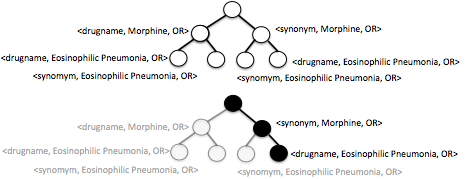
\includegraphics[scale=0.5]{p22.png}
\caption{The search space for an example with 2 queries and 2 instances. Each level of the tree represent the instances sider:12312 and sider:43434, respectively. The second tree show a solution path in the tree.} 
\vspace{-10pt}
\label{fig:sspace}
\end{figure}

Given $n$ source instances, $k$ different query types and $k$ comparable predicate pairs in $U^{*st}_A$, a naive approach would perform all $n \times k \times q$ queries to find the optimal candidate set for each instance. We show how this number of queries can be reduced through our branch-and-bound based optimization that aims to execute only a few effective queries for every source instance. 
 
\subsection{Search-based Optimization} 
The problem start by learning the schema alignments $U^{*st}_A$ from the data. Then , from this alignment, a initial set of template queries containing only attribute queries is created. Our initial search space is composed of $n \times k \times q$ queries. We conceive an iterative process where source instances are processed one by one, resulting in a tree-shaped search space where the tree nodes correspond to queries and each level of the tree represents an instance.  A path on this tree from the root to a leave indicates the queries selected for their respective instances. We will use node and query as synonyms from now on. Fig. \ref{fig:branch} overviews the search process.

\begin{figure} [h]
\vspace{-10pt}
\centering
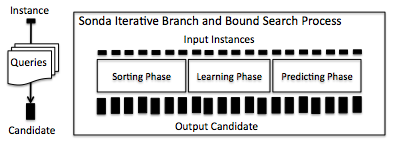
\includegraphics[scale=0.5]{p24.png}
\caption{It illustrates each intermediary step during the branch and bound search: sorting, learning and predicting. These phases differ on the branch mechanism used. } 
\vspace{-10pt}
\label{fig:branch}
\end{figure}

\subsubsection{Query Optimal Criteria} 

The goal of the optimization is to execute less queries as possible to determine the optimal one, as defined below:
\begin{definition}[Optimization Goal] Given a set of instances S and a set of template queries $Q =\{q_1,..., q_n\}$ and for every instance $s_i \in S$ exists a set of evaluated queries $Q^e_{s_i} \subset Q$, where $q^o_{s_i} \in Q^e_{s_i}$ is a optimal query for $s_i$, then the optimization goal is to minimize:
\[
{\arg \min} \bigcup_{s_i \in S}|Q^e_{s_i}| \land
{\arg \min} \bigcup_{s_i \in S} |q^o_{s_i}| 
\]
\end{definition} 

The optimal query for an instances can only be determined by evaluating all possible queries; however, to minimize the number of queries evaluated is one of the optimization goals. Both goals can be achieved simultaneously by making use of heuristics that helps to determined whether or not is necessary to evaluate a query.

Regarding the optimality of a query, the challenge is to select for each source instance the one fast query (few fast queries) needed to produce all and only the correct candidates. Thus, a query can be characterized by two dimensions, namely its \emph{execution time} and the \emph{optimality of its results}. As both criteria of optimality is not known, we propose a \emph{cardinality-based and time-based heuristics} that can estimate those criteria:

\begin{definition}[Cardinality Based Heuristic] The most optimal query is the one that yields exactly one candidate while queries with no results or too many results are less optimal. 
\end{definition} 
\begin{definition}[Time Efficiency Heuristic] A query is is optimal if it is time efficient.
\end{definition} 
The time efficiency heuristic captures the intuition queries that retrieves less elements are faster. While they are rather aggressive heuristics that are exclusively focused on reducing the number of candidates (not taking into account whether they are correct or not), we show it performs well in the experiments. 

Regarding the optimality of a the number of queries evaluated, not all queries need to be evaluate, because queries may produce subset of each other, intersecting candidate sets or even empty sets. For instance, suppose that the OR queries are superset of all other query types; consequently, a query OR cannot reduce the cardinality of a query AND, thus, it do not need to be evaluated if AND query retrieve a non-empty set. Complementary to this intuition, two queries that produces disjoint sets are both candidates to be optimal, because we cannot predict in which set are the correct matches (e.g. the query constructed from \verb+rdf:label+ retrieves candidates of type \verb+Ingredient+ while the query constructed from \verb+drugs:drugname+ retrieve \verb+Drugs+). These dependencies between template queries can be learned and used to skip the evaluation of subsequent queries.  Below we define an heuristic to capture this idea.

\begin{definition}[Candidates Intersection Heuristic] Given two distinct template queries $q_i$ and $q_j$, where $|q_i| > 0$ and $|q_j| > 0$,  if $q_i \cap q_j = \emptyset$, then their optimal candidate set is given by $q_i \cup q_j$, otherwise, the query that with smaller cardinality is optimal.
\end{definition}  

The process on which the optimization task takes place is described next.

\subsection{Best-First Search With Branch-and-Bound Pruning} 
 
Based on these heuristics, we use best-first search with branch-and-bound pruning~\cite{DBLP:journals/jacm/DechterP85} to execute only the best queries in the search space. The overall procedure is presented Alg.~1, which has three main components. It has a \emph{bounding policy}, which decides when to stop the whole process. The \emph{branching policy} determines the visit order of nodes within every level and when to move to a next level, based on cardinality and time estimates. Further, a classifier helps the branching policy to decide whether to skip certain queries or not. 

\textbf{Branching}. It is a breadth-first search procedure that processes queries associated with the source instance of the current level before moving to the next instance in the next level. In every level, this search is guided by the branching policy, which always selects the node that is best w.r.t.~ time and cardinality dimensions. More precisely, it chooses the one with lowest cardinality and among those not distinguishable in terms of that, it chooses the one that requires less time (based on the estimated values discussed before). 

According to the cardinality-based  this policy indicates to stop and to move to the next level when a node with cardinality 1 is visited (because there are no better queries than this).  However, according to the candidates intersection heuristic, an optimal candidate set is the union of non-empty and non-intersection optimal queries. We observed that non-intersecting queries occurs only for template queries build from different target predicates. Therefore, the cardinality-based is applied on set of template queries that share the same target predicate. For a N different target predicates, at least N queries are performed per instances. Once the optimal queries are found for each those sets, the search moves on to the next level. However, this process can be further optimized, by merging sets where their optimal queries produce intersecting results. To so, we apply a predictor that learns to predict from the history of queries processed in a previous levels, whether exist intersection optimal queries and which are those queries. 

\textbf{Query Predictor}. 
The predictor uses the candidate intersection heuristic to decide if a query should be evaluated or not. To exploit this, we train a classifier, which given a sequence of queries, predicts if the current node has lower cardinality than any other previous queries. Beside of that, it also predicts, if the results of current query does not intersect with the result of any other previous query. Therefore, the current query are evaluated only if any of these two conditions are satisfied.  While the branching policy can help to find optimal candidate sets, the predictor help to reduce the number of queries evaluated per level; in this way, we achieve the optimization goal.

\textbf{Bounding}. While the branching policy determines the next node to evaluate (and to stop processing one level when the optimal query is found)  the \emph{bounding policy} decides when to stop the whole process. The search should terminate when there exist no or too few matches for the source instances. This can be decided when through many levels, empty candidates sets are obtained as results. As shown in Alg.~1, the bounding strategy is 
controlled by the parameter $\gamma$. In the experiments in this paper, early termination through bounding is not used because we know in advance that matches exist between the datasets. 
\begin{algorithm}
\caption{CandidateSelection(G, G'). Find candidates for instances in $G$.}
\begin{algorithmic}
\scriptsize\tt
\STATE  sourcekeys  $\leftarrow$ FindCandidateSchema(G)
\STATE  targetkey  $\leftarrow$ FindCandidateSchema(G')
\STATE  keypairs  $\leftarrow$ AligningSchemas(sourcekeys, G, targekeys, G') 
\STATE  nodes  $\leftarrow$ BuildNodes(keypairs) 
\STATE  learning  $\leftarrow$ true
\FORALL{b in targetkeys} % Builds a classfier per target key
\STATE predictor[b] $\leftarrow$ NayveBayesClassifier.new()
\ENDFOR 
\FORALL{i in $G$} % Find candidates for each source instance
\IF { $i \geq\gamma$ and candidates = $ \emptyset $ }  %  Validate the bounding policy
\STATE  return null //Satisfied bounding policy
\ENDIF
\FORALL{node in nodes}  
\STATE  b $\leftarrow$ node.targetkey
\IF {cost[b] = 1}  
\STATE next //Satisfied branching policy 
\ENDIF
\IF {learning or predictor[b].predict(node)}  
\STATE  cost[b] = node.evaluate(i) 
\STATE  processed[b] $\leftarrow$  processsed[b] + node 
\IF {learning}  
\STATE    predictor[b].AddExample(node) //Learning Phase
\ENDIF 
\ENDIF 
\ENDFOR
\IF {$i \leq  \beta$} 
\STATE    SortNodesByElapseTime(nodes)  //Sort nodes 
\ENDIF
\IF {test error converges} 
\STATE    learning $\leftarrow$ false
\ENDIF
\IF {$i =ß \alpha$} 
\STATE  examples  $\leftarrow$ matcher(candidates)
\STATE  nodes  $\leftarrow$ updateNodes(examples) 
\STATE    learning $\leftarrow$ true
\ENDIF
\STATE  candidates[i] $\leftarrow$ AggregateMinimalCandidatesSet(processed)
\ENDFOR 
\RETURN candidates[i]
\end{algorithmic}
\end{algorithm}

\subsection{Leaning to Predict Query Optimality} 
Preceding the \emph{Learning} Phase in the Alg. 1, we describe a \emph{Sorting}  phase, aiming to process the queries that are time efficient first. Basically, nodes are sorted by their average evaluation time. Average time and this order are computed after $\beta \%$ of the instances have been processed. This order is kept to train the predictor and also used during the Prediction phase (so that branching continues with the query that requires lesser time, given they all equal in terms of cardinality). The $\beta$ parameter can be set to be small to obtain average time simply after a few instances (we set it to $1\%$ in the experiment).
 
In the \emph{Learning} phase, the predictor is learned as a Naive Bayes classifier~\cite{Hand2001Idiots}.  It predicts whether the current node to be chosen by the branching strategy indeed has lower cardinality or do not intersect with preceding nodes results . As features, we use the  identifier of a current query and a boolean value indicating if any previous query has cardinality greater than zero (i.e. whether it was executed before). 
Recall that the branching policy applies to queries constructed for every target predicate and it moves on to next queries when it found an optimal one. Similar to that, a predictor is learned for every set of nodes that share the same target predicate and accordingly, is only used for queries that have been constructed from this target predicate. The Learning phase stops soon after three iterations have the same test error. 
When the Learning phase terminates, both the branching policy and the predictor are applied to choose and to skip query nodes, respectively.  

In the \emph{Updating} phase, new template queries are generated with a class clause. The class queries are computed after $\alpha\%$ of the instances have been processed. In this work, we fix $\alpha$ to 5\% of the instances. Then, the candidates obtained so far are input to a matcher that outputs positive and negative examples. As a matcher,  the class-based disambiguator \cite{•} is used in this work. Those generated examples are input to the algorithm that computes the class clauses. For each class clause found a new query is created by adding it to the original queries. For $q$ queries and $n$ class clauses, then $n \times q$ new queries are generated in the end. After this process, the classifier is retrained using the Leaning procedure described before. 

 
 
\section{Evaluation}

\begin{itemize}
\item Describe the datasets
\item Data preparation (indexes)
\item Describe the metrics
\item Describe alternative approaches
\item Results for candidate selection
\item Results for instance matching

\end{itemize}
In this section, we discuss how we evaluate our approach and discuss about the results. Our system Sonda was implemented in Ruby and the queries were implemented as SPARQL queries issues over alive SPARQL endpoints. Sonda is available for download at GitHub as a command line tool $\footnote{https://github.com/samuraraujo/Experiments/tree/master/experiments/ICDE2013}$, as well as all the results that we obtained. 
 
\subsection{Datasets} 

We evaluated our framework using the datasets and ground truth published by the instance-matching benchmark of the Ontology Alignment
Evaluation Initiative (OAEI) \cite{DBLP:journals/jods/EuzenatMSSS11}. We used the datasets provided in 2010 and 2011. We used the life science (LS) collection (which
includes Sider, Drugbank, Dailymed TCM, and Diseasome) and the Person-Restaurant (PR) from the 2010 collection. We excluded LinkedCT from our experiments due to known quality problem in the ground truth. We used all datasets from the 2011 collection. 

\subsection{Querying Candidates} 
We implemented the queries in our algorithm as SPARQL queries (as discussed before) and directly query a SPARQL endpoint to obtain results (limit to 30 instances per query). For that, we loaded all datasets into the OpenLink Virtuoso Universal Server (Version 6.1.5.3127), except for DBPedia, which we queried its on-line sparql endpoint. We use the default S-P-O index created by this server, and created an inverted index for literal values using the following commands:

\lstset{basicstyle=\small}
\begin{lstlisting}[ ]   
DB.DBA.RDF_OBJ_FT_RULE_ADD 
(null, null, 'index_local');
DB.DBA.VT_INC_INDEX_DB_DBA_RDF_OBJ (); 
\end{lstlisting}

We use the specific Virtuoso SPARQL implementation to have access to the index, and we limited all query results to 30 instances. This avoids the queries to retrieve too many data for non-discriminative queries. For example, in this syntax, the 4 query types EXACT, LIKE, AND, and OR are, respectively: 
\lstset{basicstyle=\small}
\begin{lstlisting}[ ]   
 SELECT DISTINCT ?s  WHERE {?s ?p  'eosinophilic pneumonia' .} 
 limit 30
 
 SELECT DISTINCT ?s ?o WHERE {?s ?p ?o .
 ?o bif:contains  '"eosinophilic pneumonia"'  . } limit 30
 
 SELECT DISTINCT ?s ?o WHERE {?s ?p ?o .
 ?o bif:contains  '"eosinophilic"AND"pneumonia"'  . } limit 30
 
 SELECT DISTINCT ?s ?o WHERE {?s ?p ?o .
 ?o bif:contains  '"eosinophilic"OR"pneumonia"'  . } limit 30
\end{lstlisting}

\subsection{Evaluation metrics and alternative approaches} 
We used standard metrics, namely Reduction Ratio (RR), Pair-wise Completeness (PP) and F1. Basically, high RR means that the candidate selection algorithm helps to focus on a smaller number of candidates, while high PP means that it could preserve more of the correct candidates. Because RR is small given the number of all possible candidates is large in this scenario, we use a normalized version of RR. In particular, these metrics are computed as follows: $PC =$ \# Correctly Computed Candidates / \# Ground Truth Candidates; $RR =$ \# Instances with Non-Empty Candidate Sets / \# All Computed Candidates; $F1 = \frac{2 * RR * PC}{ RR + PC}$. Beside these metrics, we also count the average number of queries evaluated per instance as well as overall time for accomplishing the task of finding the candidate sets. 


For comparison, we implemented the \emph{S-agnostic}~\cite{papadakis_efficient_2011} and \emph{S-based}~\cite{DBLP:conf/semweb/SongH11} approaches as discussed in Sec.~2. S-based uses only an OR query and it does not feature the branch-and-bound optimization. It requires key pairs, which are generated as in Sec.~3.1. Further, S-based applies a similarity function on the keys to further prune incorrect candidates after that have been retrieved using the OR queries. For comparison purposes, we apply this strategy to all approaches, using the same similarity function. Sonda uses four types of queries for each key pair, and employs the proposed branch-and-bound optimization to select best queries. 
%. We evaluated our approach with all functionalities that we described before (including the predictor , sorting by time, etc.).

\subsection{Candidate Selection Results} 
Table 1 shows the results. Comparing all approaches over all the 16 datasets pairs that we evaluated, Sonda achieves the best F1 score in all cases (in 96\% of the cases, to be precise), except for the NYT-Geonames pair, where S-based has best F1 result (due to high RR). 
%Sonda yields better F1 score in 96\% of the cases and also
 
\begin{center}
\begin{table*}[ht]
\centering
\scriptsize\tt
\caption{Results of the three systems over all pairs of datasets. Queries denote the total number of queries given to the system. Queries/Instance denotes the amount of queries evaluated per instance.} 
    \begin{tabular}{|c|l|c|c|c|c|c|c|c|c|c|}
        \hline
        Dataset Pairs & Systems & Queries & Queries/Instance & Learning(s) & Search(s)  & RR($\%$) & PC($\%$) &  F1($\%$) \\ \hline
 
\multirow{4}{*}{Restaurant1-Restaurant2} & SondaA           \\
											& SondaC  \\
											& S-based \\
 											& S-agnostic     \\ \hline
 											
\multirow{4}{*}{Person11-Person12} & SondaA    \\
											& SondaC  \\
											& S-based \\
 											& S-agnostic      \\ \hline

\multirow{4}{*}{Person21-Person22} & SondaA  \\
											& SondaC  \\
											& S-based \\
 											& S-agnostic       	\\ \hline 										

 \multirow{4}{*}{Sider-Tcm} & SondaA            \\
 											& SondaC  \\
											& S-based \\
 											& S-agnostic        \\ \hline
 											
\multirow{4}{*}{Sider-Dailymed} & SondaA     \\
											& SondaC  \\
											& S-based  \\
 											& S-agnostic        \\ \hline 		
 																							
\multirow{4}{*}{Sider-Drugbank} & SondaA     \\
											& SondaC  \\
											& S-based \\
 											& S-agnostic      \\ \hline 											

\multirow{4}{*}{Sider-Diseasome} & SondaA      \\
											& SondaC  \\
											& S-based   \\
 											& S-agnostic         \\ \hline 		 									

\multirow{4}{*}{Dailymed-Sider} & SondaA    & 40 & 1.42   & 101.7  & 263.1   & 98.39 & 99.37 & 98.88  \\
											& SondaC  & 40 & 1.34   & 34.35  & 210.91  & 99.87 & 99.87 & 99.87 \\
											& S-based    & 8 & 8.0   & 28.17  & 1385.41  & 96.85 & 97.99 & 97.42\\
 											& S-agnostic    & 4 & 4.0   & 16.19  & 759.43    & 96.85 & 97.99 & 97.42  \\ \hline 		

\multirow{4}{*}{Diseasome-Sider} & SondaA    & 20 & 1.85   & 12.63  & 17.78   & 97.62 & 95.35 & 96.47  \\
											& SondaC   & 20 & 1.85   & 9.1  & 13.66   & 97.62 & 95.35 & 96.47 \\
											& S-based  & 4 & 4.0   & 6.37  & 51.43   & 85.11 & 93.02 & 88.89 \\
 											& S-agnostic    & 2 & 2.0   & 2.06  & 27.34   & 85.11 & 93.02 & 88.89  \\ \hline 		 									

\multirow{4}{*}{Drugbank-Sider} & SondaA    & 40 & 5.88   & 81.49  & 208.78    & 98.61 & 99.29 & 98.95 \\
											& SondaC	   & 80 & 9.92   & 70.43  & 375.57  & 97.92 & 99.29 & 98.6 \\
											& S-based     & 8 & 8.0   & 53.9  & 273.07  & 92.76 & 99.65 & 96.08\\
 											& S-agnostic   & 26 & 26.0   & 24.56  & 281.62   & 92.46 & 99.65 & 95.92 \\ \hline 											 

\multirow{4}{*}{NYT-Geonames} & SondaA   \\
											& SondaC  \\
											& S-based    \\
 											& S-agnostic     \\ \hline 											


\multirow{4}{*}{NYT-DBPedia(Geo)} & SondaA    \\
											& SondaC  \\
											& S-based \\
 											& S-agnostic       \\ \hline 											
 		
\multirow{4}{*}{NYT-DBPedia(Per)} & SondaA   \\
											& SondaC  \\
											& S-based  \\
 											& S-agnostic       \\ \hline 											
 		
 		
\multirow{4}{*}{NYT-Freebase(Geo)} & SondaA    \\
											& SondaC  \\
											& S-based   \\
 											& S-agnostic        \\ \hline 											
 
 

\multirow{4}{*}{NYT-Freebase(Corp.)} & SondaA   & 15 & 3.02   & 30.51  & 911.26  & 78.06 & 88.27 & 82.85   \\
											 & SondaC   & 15 & 3.09   & 22.09  & 986.65  & 73.21 & 88.17 & 80.0\\
											& S-based    \\
 											& S-agnostic          \\ \hline 					
 											
\multirow{4}{*}{NYT-Freebase(Person)} & SondaA  \\
											& SondaC  \\
											& S-based      \\
 											& S-agnostic       \\ \hline 								

\end{tabular}  
\end{table*} 
\end{center}

 
\textbf{Attribute Queries}. In the NYTimes-Freebases case, Sonda achieves a considerable improvement in both RR and PC. The other approaches perform worse in this case because the comparable key pairs and queries they use are not discriminative, producing too many matching instances. Sonda also considers many comparable key pairs, thereby ensuring high PC (reflecting recall). However, not all queries generated from them are used to obtain candidates but only optimal ones found during the process. This helps to balance PC with RR (reflecting precision). 

For Sider-Dailymed, we could not obtain the results for S-agnostic because it took more than 10,000 seconds to compute it. This may be attributed to the fact that the Dailymed dataset contains a large number of textual attributes and the queries generated by S-agnostic are evaluated over all these attributes, resulting in a large number of disk accesses.

\textbf{Class Queries}. The RR in $Sonda_C$ was higher than in $Sonda_A$ for a few cases (DBPedia, Freebase and Geoenames). it indicates that the class clauses indeed make the queries more precise because it select exactly the class of target instances. However, a little increase on time can be observed in $Sonda_C$, mainly due to a higher number of queries that were considered in this version.

\begin{center}
\begin{table*}[ht]
\centering
\scriptsize\tt
\caption{Sonda F1-measure (between precision and recall) compared to ExampleDriven and other tools that participate on the OAEI 2011 benchmark.} 
\begin{tabular}{|c|c|c|c|c|c|c|c|}
\hline
Dataset  &  SondaA  &  SondaC & KnoFuss+GA & AggreementMaker & SERIMI & Zhishi.links & ExampleDriven\\ \hline
DBPedia - Geo. & 0 & 0  & 0.89 & 0.69 & 0.68 & 0.92 & 0 \\ \hline
DBPedia - Org. & 0& 0 & 0.92 & 0.74 & 0.88 & 0.91 & 0\\ \hline
DBPedia - People & 0 & 0 & 0.97 & 0.88 & 0.94 & 0.97 & 0\\ \hline
Freebase - Geo. & 0 & 0 & 0.93 & 0.85 & 0.91 & 0.88 & 0\\ \hline
Freebase - Org. & 0.87 & 0.87 & 0.92 & 0.80 & 0.91 & 0.87 & 0\\ \hline
Freebase - People & & 0 0 & 0.95 & 0.96 & 0.92 & 0.93 & 0\\ \hline
Geonames & 0 & 0  & 0.90 & 0.85 & 0.80 & 0.91 & 0\\ \hline
Average & 0 & 0  & 0.93 & 0.85 & 0.89 &  0.92 & 0\\ \hline											 
\end{tabular}  
\end{table*} 
\end{center}

\begin{center}
\begin{table*}
\centering
\scriptsize\tt
\caption{Sonda  F1-measure (between precision and recall) compared ExampleDriven and  other tools that participate on the OAEI 2010 benchmark.} 
\begin{tabular}{|c|c|c|c|c|c|c|}
\hline
Dataset &  SondaA &  SondaC & SERIMI & ObjectCoref & Rimon & ExampleDriven \\ \hline
Sider-Dailymed & 0 & 0   & 0.66 & - & 0.62  & 0\\ \hline
Sider-Diseasome & 0& 0   & 0.87 & - & 0.45 & 0\\ \hline
Sider-Drugbank & 0 & 0  & 0.97 & - & 0.50  & 0\\ \hline
Sider-TCM & 0 & 0  & 0.97 & - & 0.79 &  0\\ \hline
Dailymed-Sider & 0.93  & 0.94 & 0.67 & 0.70 & 0.62  & 0\\ \hline
Drugbank-Sider & 0.80  & 0.80 & 0.48 & 0.46 & -  & 0\\ \hline
Diseasome-Sider & 0.95 & 0.95   & 0.87 & 0.74 & -  & 0\\ \hline
Person11-Person12 & 0 & 0  & 1.00 & 0.99 & 1.00  & 0\\ \hline
Person21-Person22 & 0 & 0  & 0.46 & 0.95 & 0.97 & 0\\ \hline
Restaurant1-Restaurant2 & 0 & 0  & 0.77 & 0.81  & 0.88 & 0\\ \hline
 								 									 
\end{tabular}  
\end{table*} 
\end{center}


\textbf{Time Performance}. Regarding time performance, even though Sonda has more queries to evaluate, it is faster than S-based in 56\% of the cases; it is faster than S-agnostic in 37\% of the cases. Sonda could achieve these results because it uses different types of queries with different time performances. During the process, its branch-and-bound algorithm helps to select the ones that require less evaluation time (those that are more efficient than the ones used by the other approaches). In particular, we observe that less queries does not directly translate to less execution time. For instance, the OR queries for one token is 10 times slower than the EXACT and LIKE queries together for the same token. Although queries performance time may vary among RDF store implementations, Sonda processes the fastest first, a decision that is based on experiences acquired during the process. 

\textbf{Predictor Efficiency}. We can see that in all cases, Sonda achieves a considerable reduction in the number of nodes evaluated per instance. This results shows that Sonda's predictor was very efficient, selecting only a few queries per instance, as well as, very effective, selecting queries that produce near optimal PC, in most of the cases.


\subsection{Instance Matching Results} 

In this section, we compared the Sonda F1-measure (between precision and recall) with the other alternatives approaches that were evaluated over the same datasets.
%Notice that although not ideal, Sonda completed the task in a reasonable time, considering that our approach queried directly the datasets SPARQL endpoints. 
%The drawback of this approach is that there is a huge time delay due to access to disc, packing of the data in the SPARQL protocol and transferring it via the network. In the other hand, we can integrate two alive data endpoint without any configuration issues, parameter tuning, data pre-processing and indexing, in a couple of minutes or in a few hours. 

%In summary, Sonda yields better F1 score in 96\% of the cases and also, . It means Sonda is more effective in selecting the candidates compared to other approaches, and the main reason for that is attributed to the use of multiple query types and the smart selection of the queries by the branch-and-bound algorithm.


 

 
%
\section{Related Work}
%The problem of Web-scale instance matching has only been studied recently, while most of the work so far focused on the single domain context. 

%We will now briefly discuss existing work 
%along the main dimensions of attributes (or \emph{features} in general), \emph{similarity measures} and \emph{matching techniques}. Also, we will present the main directions towards \emph{Web-scale integration} and position our contributions along this line. 

%\subsection{Matching Features}
%Instances are similar and thus, are considered candidate matches if their \emph{features} are similar \cite{fellegi_theory_1969}. 
%A great variety of features have been employed 
%in order to solve this instance matching problem, 
%while instances in different settings, may be represented as different types of database records or RDF resources. Traditionally, 
%Features used are derived from flat attributes, structure information of instances (e.g. relations between RDF resources)~\cite{melnik_similarity_2002,spaccapietra_survey_2005} or semantic information. For instance, ObjectCoref \cite{hu_bootstrapping_2011} considers resources as matches if their discriminative attributes are similar. The discriminativeness is inferred from attribute characteristics captured by semantic constraints
%expressed using the Web Ontology Language, OWL), including 
%such as 
%\verb+owl:InverseFunctionalProperty+, 
%\verb+owl:FunctionalProperty+ and \verb+owl:cardinality+. While we focus on the use of flat attribute values in the experiment, SERIMI is also applicable to other features. 

%\subsection{Similarity Measures}
%Instance matching using flat features typically relies on string comparison techniques using different \emph{similarity metrics}. Character-based metrics (e.g. Jaro, Q-grams), 
% work well for detecting typographical errors. 
%token-based metrics (e.g., SoftTF-IDF, Jaccard) and 
%work well when features have many words and the arrangement of words cannot be captured by character-based metrics (e.g., ``Michael Jackson'' vs. ``Jackson, Michael''), 
%document-based similarity metrics (e.g., cosine similarity) 
%are employed when the number of tokens to be compared is large. 
%and phonetic metrics (e.g., Soundex) can deal with features that are phonetically similar. 
%, but are not at the level of character or token. 
%Numeric metrics were designed to capture the nuances of numeric features. 
%are the types which consider strings as features. Besides these string-based metrics, 
%are not able to detect similarity between synonyms, nicknames, abbreviations and acronyms (e.g, ``Big Apple'' and ``New York''). To address this, 
%there are also lexical semantic relatedness metrics \cite{han_structural_2010,budanitsky_evaluating_2006} which leverage semantic information from general knowledge sources (e.g., Wikipedia) or lexical sources (e.g., WordNet).  Although there are many similarity metrics, there is no single one that applies in all cases \cite{cohen_comparison_2003}. 
%Different features have different characteristics that demand different metrics. Some authors propose that the best way to approach this problem is by 
%Learning the right metrics for the given features, and combining different metrics \cite{branting_comparative_2003} are the best strategies. Which metrics to be used is also not the focus here, where we simply employ a string-based metric for the experiment. 

%\subsection{Matching Techniques}

Several \emph{matching techniques} have been proposed to address both the efficiency and effectiveness of instance matching. Here, we will focus on related work that tackle the efficiency of the problem. A study about the effectiveness of instance matching was done in our previous work \cite{serimi}. 

\emph{Data blocking techniques} \cite{hernandez_merge/purge_1995} aims to make instance matching more efficient by reducing the number of unnecessary comparisons between records. Based on a feature that is distinctive and can be processed efficiently (also called Blocking Key Value, BKV), instances are partitioned into blocks such that potentially similar instances (i.e. candidate results to be further refined) are placed in the same block. Examples of blocking techniques include the sorted neighbourhood approach and canopy clustering \cite{mccallum_efficient_2000}. However, these techniques are focus on the single dataset settings, where the schema are homogeneous and the choice of a BKV is less problematic. 

So far, only one unsupervised blocking technique has been explicitly designed to work in the heterogeneous Web setting, where to tackle the heterogeneity between schemas, schema attributes are ignored and the BKV is simply the set of all tokens that can be extracted from the instance data~\cite{papadakis_efficient_2011}. As it does not use attribute information in the BKV, we call it as schema-agnostic blocking. However, the limitation of this approach is known, it may yield too many candidates because it looses valuable attribute information, which would form more discriminative keys. There is a recent work \cite{DBLP:conf/semweb/SongH11} focused on this setting that uses the attribute information, and its values, in the BKV. However, the BKV are manually defined in this approach. So far, there is no unsupervised approach that make use of both attribute-value in the BKV. Notice that differently from the single dataset setting, in the multiple datasets setting, we need to align BKV from different sources, so that we can use information from the source key to select candidates based on the target key. This is one gap that we tackle in our approach. 

%This approach differs from the single-domain techniques in that instead of using specific attributes, it simply uses tokens from all attributes. Thus, it can deal with multiple domains and schemas because instances to be compared do not have to share common attributes (i.e. their schemas are not assumed to be same or pre-aligned).

%There are two major kinds of approaches that target the effectiveness of matching. Usually, they are employed after blocking for the disambiguation of candidate matches. There are \emph{learning-based approaches} that can be further distinguished in terms of training data and degree of supervision, respectively (i.e. supervised, semi-supervised, unsupervised \cite{bernstein_discovering_2009,Song:2011:AGD:2063016.2063058,Niu:2011:ZWC:2063076.2063091}). ObjectCoref is a supervised approach that self-learns the discriminativeness of RDF properties. Then, matches are computed based on comparing values of a few discriminative properties. RIMON is an unsupervised approach that firstly applies blocking to produce a set of candidate resources and then, uses a document-based similarity metric (cosine similarity) for disambiguating candidate resources. 
%As features, it models
%%goes beyond flat attributes to 
%an instance as a vector of terms that are extracted from the structure formed by the instance and its neighbors. 
%\emph{Collective matching} represents the other kind of approach \cite{spaccapietra_survey_2005}. It exploits the intuition that two instances are similar if their neighbors are similar. Similarity flooding \cite{melnik_similarity_2002} is a generic graph-matching algorithm that implements this intuition. 
%This algorithm was adopted to the LDW setting to deal with ontology matching \cite{wang_structure-based_2010}. 

%\subsection{Instance matching on the Web}
%Recently, different directions towards \emph{Web-scale matching} have been pursued. One prominent concept is pay-as-you-go data integration \cite{das_sarma_bootstrapping_2008}, which recognizes that in large-scale scenarios, it is not affordable to perform integration completely upfront but rather, it shall be considered as a continuous process. 
% that involves users, where integration results are incrementally obtained and refined as the system evolves. 
%In particular, Google researchers have studied keyword search-based data integration, where matching tasks are carried out during user search activities \cite{DBLP:conf/sigmod/TalukdarIP10}. Besides these general concepts, a few technical solutions have also been proposed to deal with schema and ontology matching \cite{budanitsky_evaluating_2006} in the LDW context. However, besides the blocking technique \cite{papadakis_efficient_2011} and the two preliminary works, ObjectCoref and RIMON, mentioned above, there exists no effective solution for the instance-matching problem, which specifically deal with multiple domains and schemas. 

%We target this problem setting, providing an unsupervised approach that can be used in combination with existing blocking techniques \cite{papadakis_efficient_2011} to disambiguate candidate matches. 
%%That is, we focus on the effectiveness of matching, aiming at refining candidate results previously obtained through a simple but efficient blocking technique. 
%As opposed to previous works \dtr{cite}, which are based on \emph{direct matching} of instances between the source and the target datasets based on some common attributes, the disambiguation involves only instances of the same target dataset. 
%%To the best of our knowledge, 
%%this is the first approach that 
%This enables the effective matching of instances across domains and possibly non-overlapping schemas. 

\section{Conclusions}


\bibliographystyle{IEEEtran}

\bibliography{icde}

\end{document} 